\documentclass[11pt]{article}
\ifdefined\pdftrailerid\pdftrailerid{}\fi
\ifdefined\pdfinfoomitdate\pdfinfoomitdate=1\fi
\usepackage[T1]{fontenc}
\usepackage{lmodern,amsmath,amssymb,amsthm,mathtools,microtype,booktabs}
\usepackage[margin=1in]{geometry}
\usepackage{xcolor,tikz,xurl}
\usetikzlibrary{arrows.meta,positioning}
\usepackage[colorlinks=true,linkcolor=blue!45!black,citecolor=blue!45!black,urlcolor=blue!45!black]{hyperref}
\hypersetup{pdftitle={Velocity-Field Detection of Computation in Forced Navier-Stokes Flows},pdfauthor={OpenAI}}
\newcommand{\articleid}[1]{{\def\UrlBreaks{\do-}\path{#1}}}
\newtheorem{theorem}{Theorem}[section]
\newtheorem{lemma}[theorem]{Lemma}
\newtheorem{proposition}[theorem]{Proposition}
\newtheorem{corollary}[theorem]{Corollary}
\theoremstyle{definition}
\newtheorem{definition}[theorem]{Definition}
\theoremstyle{remark}
\newtheorem{remark}[theorem]{Remark}
\newcommand{\R}{\mathbb R}
\newcommand{\T}{\mathbb T}
\newcommand{\Z}{\mathbb Z}
\newcommand{\N}{\mathbb N}
\newcommand{\dd}{\,\mathrm d}
\newcommand{\eps}{\varepsilon}
\DeclareMathOperator{\diver}{div}
\DeclareMathOperator{\supp}{supp}
\DeclareMathOperator{\dist}{dist}
\title{Velocity-Field Detection of Computation in Forced Navier--Stokes Flows}
\author{OpenAI}
\date{September 27, 2026}
\begin{document}
\maketitle
\begin{abstract}
We construct smooth forces for three-dimensional incompressible
Navier--Stokes flow, from rest at any fixed positive computable viscosity,
whose velocity field detects whether a prescribed machine halts.
On the unit flat torus, a pointwise test of the third velocity component
uses successively shorter stirring intervals in a fixed spatial region.
On $\R^2\times\T$, an integral test uses an expanding array of translation
regions and a force with globally bounded mixed derivatives.
The vertical velocity solves an advection--diffusion equation: short
bursts control its pointwise error in the first construction, and a
moving cutoff controls the total escaped mass in the second.
\end{abstract}

\section{Observing the velocity rather than a particle}\label{sec:introduction}

A material observer follows one marked fluid particle. An Eulerian
observer instead examines the velocity at a time, without remembering
which particle reached which point. The distinction matters for
computation. A smooth flow can transport an exact tape encoding, but a
velocity component that carries the same information is also diffused
by viscosity. We ask whether a fixed test of the velocity can still
detect halting when the fluid starts at rest.

Write $\T=\R/\Z$. On either $\Omega=\T^3$ or
$\Omega=\R^2\times\T$, we use the flat metric and the equations
\begin{equation}\label{eq:NS}
 \partial_tu+(u\cdot\nabla)u=-\nabla p+\nu\Delta u+f,
 \qquad \diver u=0,\qquad u(0)=0.
\end{equation}
The viscosity $\nu>0$ is fixed and computable. The input consists of a
deterministic Turing machine and a finite input word. An effective force
prescription is a finite program evaluating $f$ and each requested mixed
derivative, to any rational error, at computably supplied space-time
arguments. It also gives the finite derivative bounds used in the
construction. There is no computational complexity requirement.

We use two fixed observations. On $\T^3$, with coordinates $(x,y,z)$,
the event is
\begin{equation}\label{eq:torus-event}
 \exists t\ge0\ \exists (x,y,z),\quad
 1/32<y<1/8,\qquad u_3(t,x,y,z)>\tfrac12.
\end{equation}
On $\R^2\times\T$, with coordinates $(X_1,X_2,z)$, it is
\begin{equation}\label{eq:plane-event}
 \exists t\ge0,\qquad
 \int_{\{X_2>0\}\times\T}u_3(t,X,z)\dd X\dd z>\tfrac12.
\end{equation}
All integrals over a torus coordinate use one period and normalized
Lebesgue measure. We specify the solution classes before the theorem.
A classical competitor has continuous velocity, time derivative, spatial
derivatives through order two, pressure and pressure gradient on every
finite closed time cylinder, and satisfies the equations pointwise.
On the torus its pressure is periodic and has mean zero.
On $\R^2\times\T$ they additionally satisfy, for every finite $T$,
\begin{equation}\label{eq:comparison-class}
 \begin{gathered}
 u\in C([0,T];H^2)\cap C^1([0,T];L^2),\qquad
 p\in C([0,T];H^1),\\
 \sup_{[0,T]\times\Omega}(|u|+|\nabla u|)<\infty.
 \end{gathered}
\end{equation}
The pressure condition on the noncompact domain fixes the additive
spatial constant. Smoothness at time zero means one-sided smoothness.

\begin{theorem}\label{thm:main}
For each positive computable $\nu$, a machine and a finite input
effectively determine each of the following two forces.
\begin{enumerate}
\item On $\T^3$, a smooth force has a unique global smooth solution
in the torus class above, with pressure zero, for which
\eqref{eq:torus-event} holds exactly when the machine halts.
The force is supported in $K\times\T$ for a compact
$K\subset(0,1)^2$ independent of time. Its derivatives are bounded on every finite time
interval; their bounds may grow with that interval.
\item On $\R^2\times\T$, a smooth force and all its mixed derivatives
are globally bounded. On each finite time interval its horizontal
support is compact. It has a unique global smooth solution in
\eqref{eq:comparison-class}, with pressure zero and integrable
nonnegative third component. Event~\eqref{eq:plane-event} holds exactly
when the machine halts.
\end{enumerate}
The sets and thresholds in both observations are independent of the
machine and input. The compact set $K$ in the first construction may
depend on that instance, but is independent of time. Both force prescriptions install all the required
local instructions, without executing the selected computation.
\end{theorem}

The two conclusions pay for diffusion in different ways. The first
keeps the horizontal mechanism inside one chart and speeds up its
later tests. Its force need not be bounded uniformly for infinite time.
The second keeps the amplitudes and all mixed derivatives bounded by
allowing the horizontal geometry to expand. It makes no claim of a
single compact support for all time or of uniformly bounded total
kinetic energy. Neither construction requires a solenoidal force or a
mean-zero force. These qualifications are part of the mathematical
distinction between the regimes.

The descriptions specify exact computable forces through arbitrarily
accurate evaluations. The strict observation margins proved below
concern these forces; no stability under perturbations of the force
or finite-precision replacement of its description is asserted.

\subsection{Background and the two mechanisms}

Turing proved the undecidability of whether a described machine ever
prints a designated symbol~\cite[Section~8]{Turing1936}. Replacing that
printing event by a halt gives the decision problem used here.
Moore's generalized shifts encode tapes in positional real coordinates
and represent local instructions by piecewise affine maps
\cite{Moore1990,Moore1991}. Smooth flows require injective finite-time
maps, whereas a machine may erase a symbol.
Landauer~\cite[Section~3]{Landauer1961} discusses retaining information
that an irreversible operation discards; Bennett~\cite{Bennett1973}
gives a reversible simulation that records the instruction history.
The particular one-head compiler and planar realization used here are
supplied by \cite[Lemma~3.1 and Theorem~4.1]{stationary2026}; the
diffusion estimates below are proved here.

Material-particle computation was realized by Cardona, Miranda,
Peralta-Salas and Presas in steady Euler flow on a three-sphere with a
chosen Riemannian metric~\cite[Theorem~6.1]{CardonaEtAl2021}.
Dyhr, Gonz\'alez-Prieto, Miranda and Peralta-Salas construct steady
unforced Navier--Stokes flows on suitable Riemannian three-manifolds,
using harmonic fields for the Hodge Laplacian and an adapted
metric~\cite[Theorem~A]{DyhrEtAl2026}.
These results concern trajectories of a stationary velocity, whereas
the observations here test the evolving velocity itself.

Velocity-space observation has a direct predecessor in the work of
Cardona, Miranda and Peralta-Salas~\cite{CardonaMirandaPeraltaSalas2022}.
Their construction uses the unforced incompressible Euler evolution on
a constructed high-dimensional compact Riemannian manifold; computation
is observed by entry into an open set of divergence-free velocity
fields. Here the geometry is flat and three-dimensional, the viscosity
is positive, and the initial velocity is zero. The machine and input
enter a prescribed external force, and the observations are the
pointwise and integral tests above. These differences distinguish the
present problem from both stationary-particle and Euler velocity-space
computation.

The common analytic device is particularly simple. For a planar
divergence-free field $a(t,Y)$ and a scalar $w(t,Y)$, the three-dimensional
velocity $(a,w)$ is divergence free when it is independent of $z$.
Its third equation is an advection--diffusion equation. We prescribe its
source and the horizontal force, and then solve for $w$. Thus the unknown
velocity is not concealed in a force formula.

In the torus construction, each block injects a very small bump of height
one at the initial machine code and runs a longer prefix of the planar
processor. A short physical duration keeps diffusion close to pure
transport, while a long heat-only interval makes older bumps small.
A halting run carries a fresh bump to the detector. In a nonhalting run,
the entire transported bump remains separated from it, so even its
diffusive tail stays below the threshold.

For bounded forcing, an initial impulse creates scalar mass one.
The horizontal field translates large squares between integer addresses
for all possible configurations. Longer and larger gates keep every
force derivative bounded. A cutoff moving with the chosen address
cancels transport exactly; its Laplacian measures the diffusion loss.
Choosing the gate radii fast enough makes the sum of those losses less
than $1/24$.

Section~\ref{sec:scalar-structure} establishes the scalar reduction and
the solution convention. Section~\ref{sec:compact} proves a parameterized
injection, stirring and waiting theorem, including two quantitative
specializations. Section~\ref{sec:compact-application} applies it to the
fixed torus detector. The expanding-address construction and its mass
estimate appear in Section~\ref{sec:bounded}. The classical background
for the maximum principle and parabolic kernels is described, for
example, by Aronson~\cite{Aronson1968}; all constants and comparison
arguments needed for detection are included below.

\section{A scalar component of a viscous velocity}\label{sec:scalar-structure}

Let $Y$ range over $\T^2$ or $\R^2$. Suppose $a(t,Y)$ is divergence
free, and prescribe the horizontal residual and the vertical source by
\begin{equation}\label{eq:triangular-force}
 F=\partial_ta+(a\cdot\nabla_Y)a-\nu\Delta_Ya,
 \qquad f(t,Y,z)=(F(t,Y),h(t,Y)).
\end{equation}
If
\begin{equation}\label{eq:scalar}
 \partial_tw+a\cdot\nabla_Yw=\nu\Delta_Yw+h,
 \qquad w(0)=0,
\end{equation}
then $U=(a,w)$, $p=0$, satisfies~\eqref{eq:NS}, provided $a(0)=0$.
Indeed $\diver U=\diver_Ya$, all $z$ derivatives vanish, and the
horizontal and vertical equations are exactly
\eqref{eq:triangular-force} and~\eqref{eq:scalar}.
Only $a$ and $h$ occur in the force prescription.

We will construct the scalar solution in each setting, including its
behavior at infinity in the noncompact case. Once it belongs to the
stated class, uniqueness is the classical difference-energy argument
\cite[Section~18]{Leray1934}, in the precise form proved in
\cite[Lemma~3]{entry2026}. To display its use, let $v$ be a competitor,
$e=v-U$, and $q$ the pressure difference. Then
\[
 \partial_te+(v\cdot\nabla)e+(e\cdot\nabla)U
       =-\nabla q+\nu\Delta e,
\]
and
\begin{equation}\label{eq:uniqueness}
 \frac12\frac{d}{dt}\|e\|_2^2+\nu\|\nabla e\|_2^2
       \le\|\nabla U\|_{\infty,\mathrm{op}}\|e\|_2^2.
\end{equation}
Periodic integration proves this on the torus. On $\R^2\times\T$,
insert a horizontal cutoff with gradient $O(R^{-1})$. The transport,
pressure and viscous boundary errors are bounded respectively by
\[
 C R^{-1}\|v\|_\infty\|e\|_2^2,\quad
 C R^{-1}\|q\|_2\|e\|_2,\quad
 C R^{-1}\|\nabla e\|_2\|e\|_2.
\]
All terms converge by~\eqref{eq:comparison-class}; its time regularity
justifies differentiating the energy. Let $R\to\infty$ and apply
Gronwall to~\eqref{eq:uniqueness} on $[0,T]$. Since $e(0)=0$, the
velocities agree, and the pressure normalization fixes $q=0$.
This comparison gives uniqueness for the explicitly constructed data,
not existence for arbitrary three-dimensional data.

\section{Short stirring bursts on the torus}\label{sec:compact}

This section separates the diffusion argument from the construction of
a planar machine. The input is a smooth periodic planar field and a
distinguished initial point. Its orbit either enters a target at an
integer phase or stays a positive distance away at every phase. The
output is a force for which the third velocity component distinguishes
these two cases.

We first work at viscosity one. Let $V(s,Y)$ be an effectively specified
smooth divergence-free field on $\R\times\T^2$, periodic of period one
and zero on a neighborhood of every integer phase. Its flow from phase
zero to phase $s$ is denoted $\Psi_s$. Assume that effective uniform
derivative bounds are available; choose an integer $L\ge1$ such that
\begin{equation}\label{eq:processor-derivatives}
 \|D_YV\|_{\infty,\mathrm{op}},\quad
 \|D_Y^2V\|_{\infty,\mathrm{op}}\le L,
 \qquad R=4^L.
\end{equation}
All derivative norms in this section are Euclidean operator norms.
Let $p\in\T^2$ be computable and let $E\subset\T^2$ be an open target.

\begin{theorem}[Injection, stirring and waiting]\label{thm:compact-detector}
For $V,p,E$ as above, choose either of the two pairs
\begin{equation}\label{eq:two-constants}
 (d,H)=(1/32,10^9)\quad\hbox{or}\quad(1/16,10^8).
\end{equation}
There is a smooth force on $\T^3$, effectively determined by $V,p$,
for which zero initial
velocity has a global smooth solution, unique in the classical torus
class of Section~\ref{sec:introduction}, with pressure zero and
the following properties.
\begin{enumerate}
\item If $\Psi_k(p)\in E$ for some integer $k\ge0$, then
$u_3(t,Y,z)>1/2$ for some finite $t$ and some $Y\in E$.
\item If $\dist_{\T^2}(\Psi_s(p),E)\ge2d$ for every $s\ge0$,
then $u_3(t,Y,z)<1/2$ for every $t\ge0$ and $Y\in E$.
\end{enumerate}
The third component is nonnegative. At viscosity one, its total
horizontal mass is less than $10^{-11}$. The same conclusions and
threshold hold for every positive computable viscosity, with the time
and horizontal velocity rescaled as in~\eqref{eq:compact-viscosity}.
The force is supported in the union of the horizontal support of $V$
and one fixed small neighborhood of $p$, times $\T$. All smoothness and
uniqueness assertions concern every finite time interval.
\end{theorem}

The force does not depend on $E$, so no effective presentation of the
open target is required. The target enters only the two orbit tests.
Here $d$ is the clearance required between a transported bump and the
target, and $H$ is an upper bound for the heat kernel at that clearance
or after one unit of waiting. The proof establishes that bound in
Lemma~\ref{lem:heat-bounds}.
The nonhalting hypothesis concerns the entire orbit. Integer-time
separation alone would leave open a false detection during a transition.
The first numerical pair serves the fixed torus detector in
Section~\ref{sec:compact-application}; the second serves the
slow-clock application identified at the end of that section.
The scalar proof is the same for both.

\subsection{An injection and a finite computation in each block}
\label{sec:compact-blocks}

Use the effective nondecreasing smooth step
\[
 b(r)=\begin{cases}e^{-1/r},&r>0,\\0,&r\le0,\end{cases}
 \qquad \theta(r)=\frac{b(r)}{b(r)+b(1-r)}.
\]
It is zero for $r\le0$ and one for $r\ge1$, with all derivatives flat
at the endpoints. Define a fixed bump on $\R^2$ by
\[
 g(Z)=\prod_{j=1}^2\theta(2(Z_j+1))\theta(2(1-Z_j)).
\]
It lies in $[0,1]$, equals one near zero, and is supported in $[-1,1]^2$.
Let an effective integer $C\ge1$ bound its first and second derivative
norms. For $n\ge1$, put
\begin{equation}\label{eq:compact-scales}
 \begin{aligned}
 b_n&=10^{-6}(2R)^{-n},&g_n(Y)&=g((Y-p)/b_n),\\
 D_n&=2Cb_n^{-2}(1+nL)R^{3n},&
 \delta_n&=\frac1{100(1+D_n)},\qquad t_n=2n.
 \end{aligned}
\end{equation}
The width $b_n$ makes the bump's mass small and its transported support
narrow. The quantity $D_n$ is chosen to bound the Laplacian of that
transported bump; Section~\ref{sec:compact-error} verifies the bound.
The duration $\delta_n$ then makes the accumulated diffusion error
at most $2\delta_nD_n<1/16$. These are separate roles: spatial width
controls the mass and separation, while physical duration controls
the error in height.
Here $g_n$ is periodized from the small square about a lift of $p$;
the copies have disjoint supports. In particular
\begin{equation}\label{eq:bump-bounds}
 \|\nabla g_n\|_\infty\le Cb_n^{-1},\qquad
 \|D^2g_n\|_\infty\le Cb_n^{-2},\qquad
 \int_{\T^2}g_n\le4b_n^2.
\end{equation}

Block $n$ injects this bump over time $\delta_n$, runs $n$ complete
periods of $V$ over another time $\delta_n$, and then waits for the
next block. In particular, its heat-only wait has length
$2-2\delta_n>1$. The time diagram in Figure~\ref{fig:blocks} shows the
roles of these intervals; their plotted lengths are schematic.

\begin{figure}[ht]
\centering
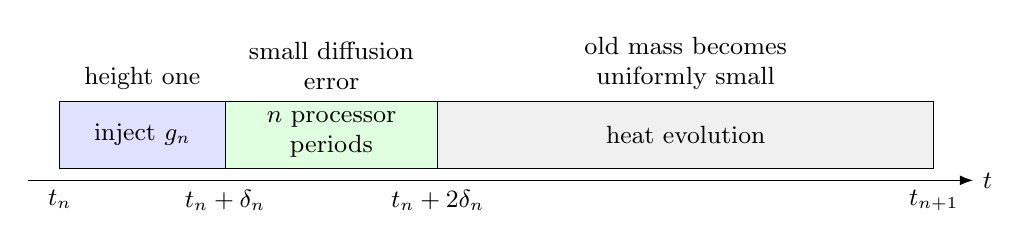
\begin{tikzpicture}[x=1cm,y=1cm,>=Latex,font=\small]
\draw[->] (0,0)--(12,0) node[right] {$t$};
\draw[fill=blue!12] (0.4,.15) rectangle (2.5,1.0);
\draw[fill=green!12] (2.5,.15) rectangle (5.2,1.0);
\draw[fill=gray!12] (5.2,.15) rectangle (11.5,1.0);
\node at (1.45,.58) {inject $g_n$};
\node[align=center,text width=2.4cm] at (3.85,.58) {$n$ processor\\periods};
\node at (8.35,.58) {heat evolution};
\node[below] at (.4,0) {$t_n$};
\node[below] at (2.5,0) {$t_n+\delta_n$};
\node[below] at (5.2,0) {$t_n+2\delta_n$};
\node[below] at (11.5,0) {$t_{n+1}$};
\node[above] at (1.45,1.03) {height one};
\node[above,align=center,text width=2.4cm] at (3.85,1.03) {small diffusion\\error};
\node[above,align=center,text width=4.8cm] at (8.35,1.03) {old mass becomes uniformly small};
\end{tikzpicture}
\caption{One torus block. Fresh scalar is injected at the initial code,
then transported through a longer finite prefix. The wait exceeds one
unit of heat time. The two active intervals are much shorter than the
wait; their relative sizes in the diagram are not to scale.}
\label{fig:blocks}
\end{figure}

Let $V_0$ be the single period of $V$ extended by zero outside $[0,1]$.
The phase collars make this extension smooth. Prescribe
\begin{equation}\label{eq:compact-program}
 \begin{split}
 s_n(t)&=n(t-t_n-\delta_n)/\delta_n,\\
 a(t,Y)&=\sum_{n\ge1}\frac n{\delta_n}
                  \sum_{j=0}^{n-1}V_0(s_n(t)-j,Y),\\
 h(t,Y)&=\sum_{n\ge1}\delta_n^{-1}
           \theta'((t-t_n)/\delta_n)g_n(Y),\\
 F(t,Y)&=\partial_ta+(a\cdot\nabla_Y)a-\Delta_Ya,
 \qquad f(t,Y,z)=(F(t,Y),h(t,Y)).
 \end{split}
\end{equation}
Each summand is supported in its indicated block. The sums are locally
finite in physical time and join smoothly at all endpoints.
Moreover $\diver_Ya=0$, $h\ge0$, and $a=h=0$ near time zero.
This prescription uses $V$ and the injection profiles, without using
the scalar that it will produce.

\subsection{Constructing the scalar and controlling old mass}

\begin{lemma}[Scalar evolution on the torus]\label{lem:torus-scalar}
For smooth $a,h$ on $[0,T]\times\T^2$ with $\diver_Ya=0$, smooth
initial data give a unique smooth solution of
$w_t+a\cdot\nabla_Yw=\Delta_Yw+h$.
Nonnegative initial data and source give $w\ge0$.
Homogeneous evolution contracts the supremum norm. On an interval
starting at $t_0$, zero initial data and $|h|\le A$ imply
$\|w(t)\|_\infty\le A(t-t_0)$.
\end{lemma}
\begin{proof}
Let $P_J$ project Fourier series onto $|k|_\infty\le J$ and solve
the finite linear system
\[
 \partial_tw_J=\Delta w_J+P_J(-a\cdot\nabla w_J+h),
 \qquad w_J(0)=P_Jw(0).
\]
For each integer $m\ge0$, differentiate through order $m$ and take
$L^2$ inner products with the corresponding derivatives of $w_J$.
The projection commutes with differentiation and drops out of these
inner products. The leading transport term has zero integral because
$\diver a=0$. In each remaining commutator a positive derivative
falls on $a$, leaving at most $m$ derivatives on $w_J$. Cauchy--Schwarz,
the finite-time bounds on $a,h$, and the nonpositive diffusion term give
\[
 \frac d{dt}\|w_J\|_{H^m}^2
       \le C_{m,T}(1+\|w_J\|_{H^m}^2).
\]
Gronwall bounds every $H^m$ norm uniformly in $J$ on $[0,T]$.

The equations bound the time derivative of every fixed Fourier
coefficient. A diagonal subsequence therefore converges uniformly in
time coefficientwise. The $H^{\ell+2}$ bound controls the differentiated
Fourier tail by a constant times
\[
 \left(\sum_{|k|_\infty>K}(1+|k|^2)^{-2}\right)^{1/2},
\]
which tends to zero in two dimensions. Hence convergence holds in
$C([0,T];C^\ell)$ for every $\ell$. The same tail argument applies
to the products and projections in the time-integrated equation.
Passing to that equation gives the scalar PDE with all spatial
derivatives. It then gives one time derivative, and repeated time
differentiation gives smoothness up to the initial time.

For comparison, subtract a proposed constant or linear upper bound
and then $\epsilon(t-t_0)$, initially allowing an arbitrarily small
strict gap as well. A first positive maximum has zero gradient,
nonpositive Laplacian and nonnegative time derivative, contradicting
the strict differential inequality. Let the gaps tend to zero. Apply
this argument also to $-w$ and to a difference of solutions. It proves
the bounds, positivity and uniqueness.
\end{proof}

Apply the lemma to~\eqref{eq:compact-program} with $w(0)=0$.
Solutions on finite intervals agree by uniqueness, giving a global
smooth nonnegative scalar. The velocity $(a,w)$ with pressure zero
is the unique three-dimensional solution by
Section~\ref{sec:scalar-structure}. Integrating the scalar equation
and using~\eqref{eq:bump-bounds} gives
\begin{equation}\label{eq:small-mass}
 0\le\int_{\T^2}w(t,Y)\dd Y
 \le M_0:=\sum_{n\ge1}4b_n^2
 =\frac{4\cdot10^{-12}}{4R^2-1}<10^{-11}.
\end{equation}
Thus infinitely many height-one injections still have very small total
mass. The heat kernel converts this mass bound into control of their
older contributions.

\begin{lemma}[Two explicit heat bounds]\label{lem:heat-bounds}
For either $(d,H)$ in~\eqref{eq:two-constants}, the unit two-torus
heat kernel satisfies
\begin{equation}\label{eq:heat-bound}
 K(\tau,Z)\le H
 \quad\hbox{if }\tau\ge1
 \quad\hbox{or}\quad\dist_{\T^2}(Z,0)\ge d.
\end{equation}
\end{lemma}
\begin{proof}
Periodizing the planar Gaussian gives
\[
 K(\tau,Z)=\frac1{4\pi\tau}
       \sum_{k\in\Z^2}e^{-|Z+k|^2/(4\tau)}.
\]
Its convolution solves the heat equation and tends uniformly to smooth
initial data as $\tau\downarrow0$, so uniqueness identifies it as the
heat kernel. Choose $Z\in[-1/2,1/2]^2$. The sup-norm shell
$|k|_\infty=j$ has $8j$ points and $|Z+k|\ge j/2$ for $j\ge1$.
Consequently
\[
 \sum_{k\in\Z^2}e^{-|Z+k|^2/8}
 \le1+8\sum_{j\ge1}j e^{-j/32}<10^4.
\]
For the last inequality, $e^{-1/32}\le32/33$ and
$\sum j q^j=q/(1-q)^2$ give an upper bound $1+8\cdot1056<10^4$.
For $0<\tau\le1$ and distance at least $d$, split each Gaussian
factor in half. One half satisfies
$\tau^{-1}e^{-d^2/(8\tau)}\le8/d^2$; summing the other halves
uses the preceding estimate. Thus
\[
 K(\tau,Z)\le\frac{8\cdot10^4}{4\pi d^2},
\]
which is less than $10^9$ for $d=1/32$ and less than $10^8$ for
$d=1/16$. At time one the same shell estimate applies without a
distance restriction; the maximum principle extends its upper bound
to all later times.
\end{proof}

Before block $n>1$, there has been more than one unit of heat-only
evolution. Therefore
\begin{equation}\label{eq:old-mass}
 0\le w(t_n,\cdot)\le HM_0;
\end{equation}
for $n=1$ the scalar is zero. From $t_n$ to $t_{n+1}$, linearity
splits $w=w^{\mathrm{old}}+w^{\mathrm{new}}$. The old part has
initial value $w(t_n)$ and no source, so remains between zero and
$HM_0$. The new part starts at zero and receives just the current
injection. It remains to estimate this new part near its transported
bump and away from it.

\subsection{A controlled diffusion error during the burst}\label{sec:compact-error}

The variational equations for $\Psi_s$ give, for $0\le s\le n$,
\begin{equation}\label{eq:flow-bounds}
 \|D\Psi_s^{\pm1}\|_\infty\le e^{Ln}\le R^n,
 \qquad
 \|D^2\Psi_s^{\pm1}\|_\infty
       \le nLe^{3Ln}\le nLR^{3n}.
\end{equation}
For the first bound, differentiate the flow once and use Gronwall.
The second variation has zero initial data, linear coefficient at
most $L$, and source at most $L$ times the square of the first
variation. Variation of constants bounds it by
$\int_0^s e^{L(s-r)}Le^{2Lr}\,dr$, and hence by $nLe^{3Ln}$.
The inverse is the flow of $-V(s-r,\cdot)$ over the reversed interval,
which obeys the same derivative bounds. These estimates are uniform
over all initial points; they do not require following the selected
machine execution.

During the two active intervals of block $n$, define the scalar that
would evolve without diffusion:
\begin{equation}\label{eq:inviscid-reference}
 w^0(t,Y)=
 \begin{cases}
 \theta((t-t_n)/\delta_n)g_n(Y),
                 &t_n\le t\le t_n+\delta_n,\\
 g_n(\Psi_{s_n(t)}^{-1}(Y)),
                 &t_n+\delta_n\le t\le t_n+2\delta_n.
 \end{cases}
\end{equation}
The endpoint flatness and phase collars make these expressions agree
smoothly. They satisfy $w^0_t+a\cdot\nabla w^0=h$.
The chain rule and~\eqref{eq:flow-bounds} bound the Hessian during
stirring by
\[
 Cb_n^{-2}R^{2n}+Cb_n^{-1}nLR^{3n}.
\]
Taking the trace costs at most two. Since $b_n<1$ and $R\ge1$,
the result is at most $D_n$ from~\eqref{eq:compact-scales}; the
injection bound is smaller. Subtracting the inviscid equation from
the diffusive one shows that $w^{\mathrm{new}}-w^0$ has zero initial
data and source $\Delta w^0$. Lemma~\ref{lem:torus-scalar} gives
\begin{equation}\label{eq:burst-error}
 \|w^{\mathrm{new}}-w^0\|_\infty
 \le2\delta_nD_n<\frac1{50}<\frac1{16}
\end{equation}
throughout the injection and stirring intervals.

Suppose first that $\Psi_k(p)\in E$ for an integer $k\ge0$.
Choose $n\ge\max\{1,k\}$. At the stirring time with $s_n(t)=k$,
the reference at $Y=\Psi_k(p)$ equals $g_n(p)=1$. The old part is
nonnegative, so~\eqref{eq:burst-error} gives $w(t,Y)>15/16>1/2$.
This proves the first implication of Theorem~\ref{thm:compact-detector}.

Now suppose the orbit stays at distance at least $2d$ from $E$.
Every point of the reference support lies within distance
\[
 \sqrt2\,b_nR^n=\sqrt2\,10^{-6}2^{-n}<1/32\le d
\]
of $\Psi_{s_n(t)}(p)$ during stirring. The same bound follows directly
during injection. The reference support is therefore at distance at
least $d$ from $E$ at every active time. In particular, $w^0=0$
on $E$, and
\begin{equation}\label{eq:active-exclusion}
 w(t,Y)\le HM_0+1/16\qquad(Y\in E)
\end{equation}
during injection and stirring.

At the end of stirring, the reference still has this separation and,
by area preservation, has mass $\int g_n$. During the wait, the new
part is the heat evolution of that reference plus the heat evolution
of an error with supremum norm below $1/16$. The latter bound is
preserved; Lemma~\ref{lem:heat-bounds} bounds the former contribution
on $E$ by $H\int g_n$. Including the old part gives
\begin{equation}\label{eq:wait-exclusion}
 w(t,Y)\le2HM_0+1/16<1/2\qquad(Y\in E).
\end{equation}
The last inequality holds for both pairs in~\eqref{eq:two-constants}.
Before the first block $w=0$. Equations~\eqref{eq:active-exclusion}
and~\eqref{eq:wait-exclusion} cover all later times and every endpoint,
proving the second implication.

\subsection{Effective prescription and physical viscosity}

For a computably supplied $t\ge0$, choose rational $q$ with
$|q-t|\le1$ and put $N_t=\max\{1,\lceil(q+1)/2\rceil\}$.
Every summand of~\eqref{eq:compact-program} with $n>N_t$ starts after
$t$ and vanishes there with all derivatives. The remaining sum is
finite, and its $n$th term contains only $n$ translates of $V_0$.
Effective derivative bounds give $L,C$, and hence all scales.
No comparison of an exact real with a block boundary is needed:
near zero, derivatives of $b$ are polynomial factors times $e^{-1/r}$,
and $s^m e^{-s}\le(m+j)!s^{-j}$ bounds their tails effectively.
Also $b(r)+b(1-r)\ge e^{-2}$. These estimates give effective
evaluation of the smooth profiles even at undecidable endpoint
equalities. Periodic charts are evaluated by finite supersets of their
possibly active translates.

The force formula repeatedly uses the same whole-period processor,
which contains all its local branches. Increasing $n$ asks the flow
to perform more periods, not the force evaluator to determine the
visited configurations. In particular evaluation of $f$ never uses
the unknown scalar $w$.

For a positive computable physical viscosity $\nu$, set
\begin{equation}\label{eq:compact-viscosity}
 U_\nu(t,Y,z)=(\nu a(\nu t,Y),w(\nu t,Y)),\qquad
 f_\nu(t,Y,z)=(\nu^2F(\nu t,Y),\nu h(\nu t,Y)).
\end{equation}
Every horizontal equation acquires the factor $\nu^2$, and every
vertical term the factor $\nu$. Thus direct substitution gives
viscosity $\nu$ with pressure zero. The vertical threshold and mass
are unchanged apart from the time parameter. The time intervals
$\delta_n$ and the waits above are measured in unit-viscosity time;
their physical lengths are divided by $\nu$. Smoothness, effective
evaluation and finite-time uniqueness persist. For an arbitrary
positive real $\nu$, the same formulas have the corresponding
oracle-relative interpretation. This completes the proof of
Theorem~\ref{thm:compact-detector}.

\section{The fixed torus detector}\label{sec:compact-application}

We now supply the geometric input and complete the first part of
Theorem~\ref{thm:main}. The planar processor theorem in
\cite[Theorem~4.1]{stationary2026} effectively constructs from a machine
and its input a smooth one-periodic Hamiltonian field $V$ on $\T^2$,
zero in phase collars, supported in a compact subset of the open unit
square. Its initial point is exactly $p=(1/4,1/4)$. At integer phases
the orbit follows the full closed rectangles of the reversible
compiler. If the machine halts, an integer-phase point enters
\[
 E=\{(x,y):1/32<y<1/8\}
\]
at distance at least $1/32$ from its boundary. If the machine does
not halt, the complete trajectory, including each intermediate
routing segment, satisfies $3/16\le y\le7/8$.
The circle distance from this corridor to $E$ is at least $1/16$.
The same theorem supplies effective global first- and second-derivative
bounds, and its quantitative flow statement supplies both forward and
inverse bounds; alternatively~\eqref{eq:flow-bounds} follows directly
from~\eqref{eq:processor-derivatives}.

Take $d=1/32$ and $H=10^9$. The nonhalting distance is at least $2d$,
and the integer halting entry satisfies the other alternative in
Theorem~\ref{thm:compact-detector}. Its two implications are therefore
exactly the equivalence in~\eqref{eq:torus-event}. All injections are
inside a fixed small square about $(1/4,1/4)$, and the horizontal
force uses only derivatives and products of $V$. Thus their union
is contained in one compact $K\subset(0,1)^2$, fixed for this
prescription. The pressure is zero and the scalar construction gives
the global smooth solution from rest. This proves the first part of
Theorem~\ref{thm:main}.

The second quantitative specialization of the detector theorem is
useful for a planar realization whose nonhalting orbit stays in
$1/8<x<3/8$ and whose target is $2/3<x<5/6$.
The infimum circle separation is at least
\[
 \min\{2/3-3/8,\,1+1/8-5/6\}=7/24>1/4.
\]
Consequently the hypotheses hold with $d=1/16$, $H=10^8$, whenever
that realization also supplies phase collars, integer halting entry
and the derivative bounds in~\eqref{eq:processor-derivatives}.
This is a direct specialization of the proved scalar theorem; it
does not require importing an alternative geometric construction
into the present proof.
This specialization is applied to the planar processor of
\cite[Lemma~7.2]{slowclocks2026} in
\cite[Section~7.5]{slowclocks2026}.

\section{Bounded forcing on an expanding array}
\label{sec:bounded}\label{cbe:section}

Diffusion can also be controlled by enlarging the region that carries
each computational state.  We now use this option to keep every mixed
derivative of the force bounded.  A horizontal incompressible field
installs all possible transitions between finitely many addresses at
each stage.  A positive vertical impulse selects one address.  The
vertical velocity then obeys an advection--diffusion equation, and a
moving cutoff measures the mass that remains near the selected
computation.  The radii grow fast enough that the cumulative diffusion
loss is less than a fixed detection margin.

We prove the second part of Theorem~\ref{thm:main}, on
$\Omega=\R^2\times\T$ with the solution class
\eqref{eq:comparison-class}. The horizontal force support will be
compact on each finite interval, while the scalar has diffusion tails.
We verify those tails in the exact comparison spaces before applying
uniqueness.

\subsection{Finite addresses and their transitions}
\label{cbe:addresses}

The only computational input is the injective local compiler of
\cite[Lemma~3.1]{stationary2026}.  Its output is
a finite partial one-head table with states $i=1,\ldots,N$, tape
alphabet $\Sigma$, and an initial tape differing from the full blank
symbol at finitely many cells.  It has one terminal state, with no outgoing rule.
Its initialized run reaches that state exactly when the original
machine halts; otherwise every successive transition is defined.
Every target state fixes the displacement of its incoming rules, and
the target state together with the full written symbol identifies
the incoming rule.  The compiler first adds a nonterminal initial
step, so these assertions include an input on which the original
machine is already halted.  Its history mechanism is the reversible
recording method used by Bennett~\cite{Bennett1973}; here we use
the stated finite table, including its full-domain incoming-rule
property.

Let $b=|\Sigma|\ge2$ and assign its symbols distinct digits
$d_\alpha\in\{0,\ldots,b-1\}$, with the full blank symbol assigned
zero.  The integer
$\sum_{j\ge0}d_{\alpha_j}b^j$ encodes an eventually blank stack whose
top is $\alpha_0$.  Zero tails are interpreted as infinitely many
blanks.  For a configuration, let $x$ encode the tape strictly left
of the head, nearest cell first, and let $y$ encode the head cell and
the tape to its right.  If the rule reads $\alpha$, writes $\beta$
and enters state $i'$, then $d_\alpha=y\bmod b$, and the new stacks are
\begin{equation}\label{cbe:stack}
\begin{array}{c|cc}
\text{move}&x'&y'\\ \hline
\mathsf R&bx+d_\beta&\lfloor y/b\rfloor\\
\mathsf N&x&y-d_\alpha+d_\beta\\
\mathsf L&\lfloor x/b\rfloor&
 d_\gamma+bd_\beta+b^2\lfloor y/b\rfloor,
 \quad d_\gamma=x\bmod b.
\end{array}
\end{equation}
These formulas push and remove exactly the indicated tape symbols.

They also give an injective map on all configurations where a rule
is defined.  The target state determines which row applies.  In the
right row the lowest digit of $x'$ recovers $d_\beta$; in the stationary
row the lowest digit of $y'$ does so; in the left row the second
lowest digit of $y'$ does so, while its lowest digit recovers
$d_\gamma$.  The compiler then identifies the old state and read
symbol.  The inverses are, respectively,
\[
 (x,y)=\bigl((x'-d_\beta)/b,\,by'+d_\alpha\bigr),\qquad
 (x,y)=\bigl(x',\,y'-d_\beta+d_\alpha\bigr),
\]
and
\[
 (x,y)=\bigl(bx'+d_\gamma,\,
                  b\lfloor y'/b^2\rfloor+d_\alpha\bigr).
\]
This proves injectivity without restricting to the initialized run.

Choose $m\ge1$ effectively so that the two initial stacks are smaller
than $b^m$, and define
\begin{equation}\label{cbe:counts}
 B_n=b^{m+n},\qquad K_n=NB_n^2=K_0D^n,\qquad D=b^2.
\end{equation}
Every update with $0\le x,y<B_n$ has $0\le x',y'<B_{n+1}$.
For the largest expression, in the left row,
\[
 y'\le(b-1)+b(b-1)+b^2(B_n/b-1)=bB_n-1.
\]
All other bounds follow directly from \eqref{cbe:stack}.
At level $n$, give the triple $(i,x,y)$ the address
\begin{equation}\label{cbe:address}
 k=1+x+B_ny+B_n^2(i-1),\qquad 1\le k\le K_n.
\end{equation}
Integer division recovers the triple.  Thus every address with a
defined instruction determines one target address $k'$ at level
$n+1$, and distinct defined addresses have distinct targets.
Only this one-step lookup is used to prescribe the force.

\subsection{Disjoint translation gates at increasing scales}
\label{cbe:gates}

We now assign each address a square and move all defined source
squares to their targets simultaneously.  Three successive motions
keep the squares separated: descent along source columns, horizontal
motion along private rows, and vertical motion along target columns.

Use the smooth step $\theta$ from Section~\ref{sec:compact-blocks}, and put
\[
 \Theta(r)=\theta(2r-1/2).
\]
The function $\Theta$ makes its transition between
$1/4$ and $3/4$.  Introduce the scales
\begin{equation}\label{cbe:scales}
\begin{aligned}
 C_*&=3000,&\Lambda&=4D,
 &R_0&=1024C_*(1+\nu)\Lambda(K_0D+2),\\
 R_n&=R_0\Lambda^n,&S_n&=16R_n,
 &T_n&=S_{n+1}(K_{n+1}+2),\\
 t_0&=1,&t_{n+1}&=t_n+T_n.
\end{aligned}
\end{equation}
The constant $C_*$ will bound the Laplacian of a cutoff at radius
$R$ by $C_*/R^2$. For scalar mass at most one, a stage of duration
$T_n$ will therefore lose at most $\nu C_*T_n/R_n^2$ from that
cutoff. The radii grow faster than the number of addresses so that
these losses form a summable series. The durations $T_n$ are long
enough for the most distant gate to move at bounded speed.
In particular $R_n,T_n\ge1$, and $t_n\ge n+1$.

Let $s_i=1$ for the terminal state and $s_i=-1$ for every other state.
An address $k$ of state $i$ has center
\[
 p_{n,k}=(S_nk,s_iS_n).
\]
The known initial configuration determines a center $p_*$ at level
zero.  It lies on the negative row.  For a defined source address $k$
at level $n$, with target $k'$ in state $i'$, put
\[
 Y_k=-(k+2)S_n,\qquad
 \theta_j(t)=\Theta\bigl(3(t-t_n)/T_n-(j-1)\bigr),
 \quad j=1,2,3.
\]
Its center path on $[t_n,t_{n+1}]$ is
\begin{equation}\label{cbe:path}
\begin{aligned}
 c_{n,k,1}(t)&=(1-\theta_2(t))S_nk
                         +\theta_2(t)S_{n+1}k',\\
 c_{n,k,2}(t)&=-(1-\theta_1(t))S_n
            +(\theta_1(t)-\theta_3(t))Y_k
                         +\theta_3(t)s_{i'}S_{n+1}.
\end{aligned}
\end{equation}
It starts at $p_{n,k}$ because every defined source is nonterminal,
and it ends at $p_{n+1,k'}$.  The supports of
$\dot\theta_1,\dot\theta_2,\dot\theta_3$ occur in successive
disjoint time slots, with stationary collars between them.

During the first slot, distinct centers have first coordinates
separated by at least $S_n$.  During the second, their private
heights $Y_k$ are separated by at least $S_n$.  During the third,
their target first coordinates are separated by at least
$S_{n+1}$, by the injectivity just proved.  The same separations
hold through the intervening collars.  If the target is nonterminal,
every vertical segment stays at or below the source row:
\begin{equation}\label{cbe:negative}
 c_{n,k,2}(t)\le-S_n\qquad(t_n\le t\le t_{n+1}).
\end{equation}

To realize one center path, set
\[
 \chi(a)=\prod_{\ell=1}^2\theta(a_\ell+3)\theta(3-a_\ell),
 \qquad \nabla^\perp=(\partial_{X_2},-\partial_{X_1}).
\]
For $c=c_{n,k}$, $G=\dot c$ and $\xi=X-c(t)$, define
\begin{equation}\label{cbe:gate}
 W_{n,k}(t,X)=\nabla^\perp
   \left[\chi(\xi/R_n)(G_1\xi_2-G_2\xi_1)\right].
\end{equation}
This field is divergence free, equals $G$ when
$|\xi|_\infty\le2R_n$, and vanishes when
$|\xi|_\infty\ge3R_n$.  The gate supports are disjoint at each
time, since their centers are separated in one coordinate by at
least $16R_n>6R_n$.
Figure~\ref{fig:translation-gates} displays the separation coordinate
in each time slot.

\begin{figure}[ht]
\centering
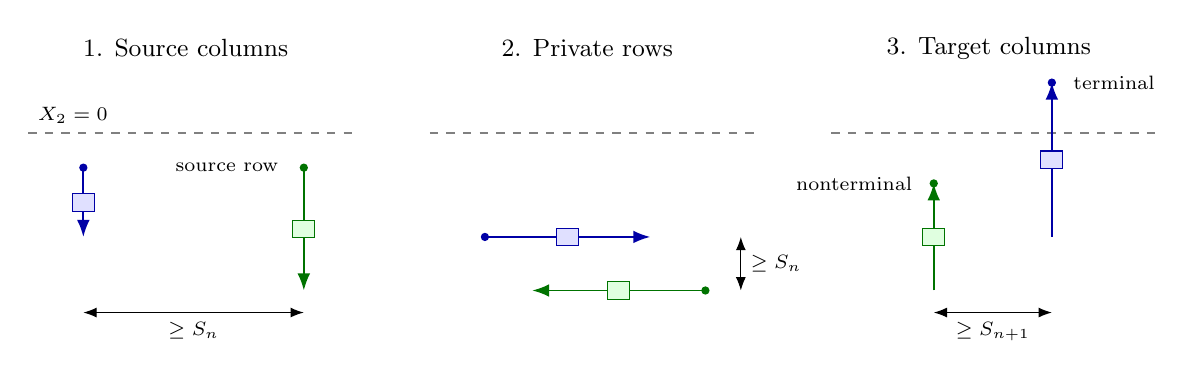
\begin{tikzpicture}[x=1cm,y=.8cm,>=Latex,font=\scriptsize,
  route/.style={line width=.7pt,->},
  first/.style={blue!65!black},
  second/.style={green!45!black},
  gateone/.style={draw=blue!65!black,fill=blue!12},
  gatetwo/.style={draw=green!45!black,fill=green!12}]
\begin{scope}
  \node[font=\small] at (2,1.35) {1. Source columns};
  \draw[dashed,gray] (0,0)--(4.2,0);
  \node[anchor=south west] at (0,0) {$X_2=0$};
  \draw[route,first] (.7,-.55)--(.7,-1.65);
  \draw[route,second] (3.5,-.55)--(3.5,-2.5);
  \fill[first] (.7,-.55) circle (1.5pt);
  \fill[second] (3.5,-.55) circle (1.5pt);
  \node[anchor=east] at (3.3,-.55) {source row};
  \draw[gateone] (.56,-1.24) rectangle (.84,-.96);
  \draw[gatetwo] (3.36,-1.665) rectangle (3.64,-1.385);
  \draw[<->] (.7,-2.85)--(3.5,-2.85);
  \node[below] at (2.1,-2.85) {$\ge S_n$};
\end{scope}
\begin{scope}[xshift=5.1cm]
  \node[font=\small] at (2,1.35) {2. Private rows};
  \draw[dashed,gray] (0,0)--(4.2,0);
  \draw[route,first] (.7,-1.65)--(2.8,-1.65);
  \draw[route,second] (3.5,-2.5)--(1.3,-2.5);
  \fill[first] (.7,-1.65) circle (1.5pt);
  \fill[second] (3.5,-2.5) circle (1.5pt);
  \draw[gateone] (1.61,-1.79) rectangle (1.89,-1.51);
  \draw[gatetwo] (2.26,-2.64) rectangle (2.54,-2.36);
  \draw[<->] (3.95,-1.65)--(3.95,-2.5);
  \node[anchor=west] at (3.95,-2.075) {$\ge S_n$};
\end{scope}
\begin{scope}[xshift=10.2cm]
  \node[font=\small] at (2,1.35) {3. Target columns};
  \draw[dashed,gray] (0,0)--(4.2,0);
  \draw[route,first] (2.8,-1.65)--(2.8,.8);
  \draw[route,second] (1.3,-2.5)--(1.3,-.8);
  \fill[first] (2.8,.8) circle (1.5pt);
  \fill[second] (1.3,-.8) circle (1.5pt);
  \node[anchor=west] at (2.95,.8) {terminal};
  \node[anchor=east] at (1.15,-.8) {nonterminal};
  \draw[gateone] (2.66,-.565) rectangle (2.94,-.285);
  \draw[gatetwo] (1.16,-1.79) rectangle (1.44,-1.51);
  \draw[<->] (1.3,-2.85)--(2.8,-2.85);
  \node[below] at (2.05,-2.85) {$\ge S_{n+1}$};
\end{scope}
\end{tikzpicture}
\caption{Two installed gates in the three successive motions of one
stage (schematic, not to scale). Small squares bound instantaneous
supports. Source columns, private rows and target columns separate
simultaneous supports, although routes from different phases may cross.
Nonterminal routes stay below $X_2=0$; terminal routes ascend across it.
The squares do not represent the support of the diffusing scalar.}
\label{fig:translation-gates}
\end{figure}

Let $W=0$ on $[0,1]$, and on $[t_n,t_{n+1}]$ sum
\eqref{cbe:gate} over every level-$n$ address with a defined rule.
The sum is finite.  Every gate is zero near the time-slot endpoints,
so these formulas join smoothly, including at $t=1$.  The resulting
field has compact horizontal support on each finite time interval
and has the exact plateau property
\begin{equation}\label{cbe:plateau}
 W(t,X)=\dot c_{n,k}(t)
 \quad\hbox{whenever }|X-c_{n,k}(t)|_\infty\le R_n.
\end{equation}

Here is why the growing array costs no derivative bound.  Every
coordinate used in \eqref{cbe:path} is bounded by a fixed multiple
of $T_n$: for example,
$|Y_k|\le S_n(K_n+2)\le T_n$ and
$S_{n+1}k'\le T_n$.  Therefore, for every $j\ge1$,
\begin{equation}\label{cbe:center-bounds}
 |c_{n,k}^{(j)}(t)|\le C_j T_n^{1-j},
\end{equation}
with $C_j$ independent of $n$ and $k$.  Differentiating the potential
in \eqref{cbe:gate} writes the gate as
$A((X-c)/R_n)\dot c$ for a fixed smooth compactly supported matrix
$A$.  A spatial derivative contributes $R_n^{-1}$; time derivatives
contribute derivatives of $c$ divided by $R_n$, together with higher
derivatives of $c$.  Since $R_n,T_n\ge1$, the product and chain rules
and \eqref{cbe:center-bounds} bound each fixed mixed derivative
uniformly in $n,k$.  At most one gate contributes at a point.
The same global bounds thus hold for $W$.

\subsection{A prescribed impulse and its scalar evolution}
\label{cbe:scalar-section}

The horizontal field is now fixed.  The remaining force is a unit
vertical impulse near $p_*$.  Prescribe
\begin{equation}\label{cbe:force}
\begin{aligned}
 f_h&=\partial_tW+(W\cdot\nabla_X)W-\nu\Delta_XW,\\
 g(t,X)&=\theta'(t)\prod_{\ell=1}^2\theta'\bigl(X_\ell-(p_*)_\ell+1/2\bigr),\\
 f(t,X,z)&=(f_h(t,X),g(t,X)).
\end{aligned}
\end{equation}
All terms are prescribed independently of the unknown vertical
velocity.  The bounds for $W$ prove global boundedness of all mixed
derivatives of $f$, and its horizontal support is compact on each
finite time interval.  Moreover, $g\ge0$, its support lies in
$0\le t\le1$ and $|X-p_*|_\infty\le1/2$, and
\begin{equation}\label{cbe:impulse}
 \int_{\mathbb R^2}g(t,X)\,dX=\theta'(t).
\end{equation}

Define $\rho$ by solving
\begin{equation}\label{cbe:scalar}
 \partial_t\rho+W\cdot\nabla_X\rho
       =\nu\Delta_X\rho+g,\qquad \rho(0,X)=0.
\end{equation}
We need integrability as well as smoothness, because both the mass
test and the noncompact uniqueness argument use it.

\begin{lemma}[Smooth scalar evolution with integrable tails]
\label{cbe:scalar-lemma}
Equation \eqref{cbe:scalar} has a global smooth solution.  Every
space-time derivative is continuous in time with values in
$C_0(\mathbb R^2)\cap L^1(\mathbb R^2)$, where $C_0$ denotes
continuous functions tending to zero at infinity.  Furthermore,
\begin{equation}\label{cbe:mass}
 \rho\ge0,\qquad
 \mathcal M(t):=\int_{\mathbb R^2}\rho(t,X)\,dX=\theta(t)\le1.
\end{equation}
\end{lemma}

\begin{proof}
For $s>0$, let
$H_s(X)=(4\pi\nu s)^{-1}\exp(-|X|^2/(4\nu s))$.
Since $\operatorname{div}_XW=0$, the mild equation is
\begin{equation}\label{cbe:mild}
 \rho(t)=\int_0^t H_{t-r}*g(r)\,dr
 -\sum_{\ell=1}^2\int_0^t
       (\partial_\ell H_{t-r})*(W_\ell(r)\rho(r))\,dr.
\end{equation}
For an integer $a\ge0$, let $E_a$ be the Banach space of $C^a$
functions whose derivatives of order at most $a$ lie in $C_0\cap L^1$,
with norm
\[
 \|v\|_{E_a}=\sum_{|\alpha|\le a}
       \bigl(\|\partial^\alpha v\|_\infty
                    +\|\partial^\alpha v\|_1\bigr).
\]
Heat convolution is a contraction on each derivative norm and is
strongly continuous on $E_a$.  The latter follows from continuity
of translations in $C_0$ and $L^1$ and the approximate-identity
property of the heat kernels.  Multiplication by $W_\ell(t)$ is a
bounded operator on $E_a$, continuous in time in operator norm on
finite intervals, by the bounded derivatives of $W$.

The elementary estimate
$\|\partial_\ell H_s\|_1\le C_\nu s^{-1/2}$ shows that the linear
operator in the second term of \eqref{cbe:mild} has norm at most
$C_a\sqrt{\tau}$ on $C([0,\tau];E_a)$.  For sufficiently small
$\tau$ this is a contraction.  The same integrable kernel bound
proves continuity of the time integrals at their upper endpoints.
On a later interval one adds heat evolution of the value at its
left endpoint.  A uniform short interval length on each $[0,T]$
therefore constructs a solution on every finite interval.  Uniqueness
in $E_0$ identifies the solutions constructed for the different $a$.

Put $F=g-\operatorname{div}_X(W\rho)$.  The spatial regularity just
proved gives $F\in C([0,T];E_a)$ for every $a$, and
\eqref{cbe:mild} becomes
$\rho(t)=\int_0^tH_{t-r}*F(r)\,dr$.
For $v\in E_{a+2}$,
\[
 \frac{d}{ds}(H_s*v)=\nu H_s*\Delta v
\]
extends continuously to $s=0$ in $E_a$.  Differentiation under the
integral gives $\partial_t\rho=F+\nu\Delta\rho$ in every $E_a$.
Repeated differentiation of this identity proves the claimed time
regularity.  In particular all smoothness statements hold one-sided
at $t=0$; the source is flat there.

All terms of \eqref{cbe:mild} are absolutely integrable in space and
time.  Integrating it and using
$\int\partial_\ell H_s=0$ gives
$\mathcal M(t)=\int_0^t\theta'(r)\,dr=\theta(t)$.
For positivity, fix $T$ and set
$v_\varepsilon=\rho+\varepsilon(1+t)$.
Continuity into $C_0$ implies uniform decay of $\rho(t,X)$ as
$|X|\to\infty$ for $0\le t\le T$: the image of this compact time
interval is compact in $C_0$ and can be covered by finitely many
small sup-norm balls.  Hence $v_\varepsilon$ is positive outside
one fixed compact set.  It is also positive initially.  At a first
zero, attained inside that compact set, its time derivative is
nonpositive, its gradient vanishes and its Laplacian is nonnegative.
But its equation has source $g+\varepsilon>0$, a contradiction.
Letting $\varepsilon\downarrow0$ proves $\rho\ge0$.
\end{proof}

We can now verify the fluid equation and its solution class.  Set
\begin{equation}\label{cbe:solution}
 u(t,X,z)=(W(t,X),\rho(t,X)),\qquad p(t,X,z)=0.
\end{equation}
The divergence vanishes and $u\cdot\nabla=W\cdot\nabla_X$ on
these $z$-independent components.  Thus the horizontal equation is
the definition of $f_h$ in \eqref{cbe:force}, and the vertical
equation is \eqref{cbe:scalar}.  Both components start from zero.

On $[0,T]$, the horizontal field and its derivatives have support in
one compact set.  Every derivative of $\rho$ is continuous in both
$L^1$ and $L^\infty$ by Lemma~\ref{cbe:scalar-lemma}.
The inequality
\[
 \|v\|_2^2\le\|v\|_1\|v\|_\infty
\]
applied also to differences at two times gives continuity into
$L^2$.  Applying it to the spatial derivatives through order two
and to $\partial_t\rho$ proves exactly the velocity regularity in
\eqref{eq:comparison-class}; the same lemma gives the required bounded velocity
and gradient.  Pressure zero belongs to the stated pressure class.

The comparison argument of Section~\ref{sec:scalar-structure} now
applies in exactly the established class. In particular, its pressure
cutoff error uses $L^2$ pressure, and its velocity errors use the scalar's
integrable tails, not compact support of the scalar. It gives uniqueness
among all three-dimensional competitors in
\eqref{eq:comparison-class}. The half-plane integral is well defined by
Lemma~\ref{cbe:scalar-lemma}.

\subsection{A moving cutoff and the detection margin}
\label{cbe:detection}

We have constructed the force and its unique solution without
following the selected computation.  Only to prove the halting
equivalence do we now follow that run.  During loading put $c(t)=p_*$.
Thereafter concatenate the paths \eqref{cbe:path} corresponding to
its successive configurations, up to the first terminal endpoint
if one occurs.  Each required gate is present because of the
integer-stack bounds and the compiler's continuation property.
The paths agree at endpoints and are stationary in endpoint collars.

An explicit test function will quantify the mass retained near
$c(t)$.  On $[0,1]$ put
$P(s)=10s^3-15s^4+6s^5$, extending it by zero to the left and one
to the right.  This extension is $C^2$, takes values in $[0,1]$,
and satisfies $|P''|\le360$.  Define
\[
 A_*(s)=P(2(1+s))P(2(1-s)),\qquad
 \varphi_R(a)=A_*(a_1/R)A_*(a_2/R).
\]
Then $0\le\varphi_R\le1$, it equals one on
$|a|_\infty\le R/2$, and it vanishes for $|a|_\infty\ge R$.
The transition intervals of the two factors in $A_*$ are disjoint;
on each, the other factor equals one.  Consequently
$|A_*''|\le1440$, and
\begin{equation}\label{cbe:laplacian}
 \|\Delta\varphi_R\|_\infty\le2880R^{-2}\le C_*R^{-2}.
\end{equation}

Take $R=R_0$ during loading and $R=R_n$ during the $n$th
transition, and within each such interval put
\[
 \mathcal I(t)=\int_{\mathbb R^2}
            \varphi_R(X-c(t))\rho(t,X)\,dX.
\]
Differentiating under the integral and integrating by parts against
the compactly supported $C^2$ cutoff gives
\begin{equation}\label{cbe:moving}
\begin{aligned}
 \mathcal I'(t)
  ={}&\int_{\mathbb R^2}
       \bigl((W-\dot c)\cdot\nabla\varphi_R(X-c)
                    +\nu\Delta\varphi_R(X-c)\bigr)\rho\,dX\\
   &+\int_{\mathbb R^2}\varphi_R(X-c)g\,dX.
\end{aligned}
\end{equation}
The transport term vanishes exactly by \eqref{cbe:plateau}; during
loading both $W$ and $\dot c$ are zero.  Positivity,
$\mathcal M\le1$, and \eqref{cbe:laplacian} bound the diffusion
term below by $-\nu C_*R^{-2}$.  The loading source is supported
where $\varphi_{R_0}=1$, because $R_0\ge1$; it contributes
$\mathcal M'(t)$.  After loading the source vanishes.

There is no loss at a radius change.  Indeed
$R_{n+1}\ge2R_n$, so the new cutoff equals one on the entire support
of the previous one, with the same center at the joint.  Nonnegativity
then implies that $\mathcal I$ cannot decrease at that change.
Starting with zero mass and integrating \eqref{cbe:moving} yields,
at every time through the first terminal endpoint,
\begin{equation}\label{cbe:loss}
 \mathcal I(t)\ge\mathcal M(t)-\delta,\qquad
 \delta=\nu C_*\left(R_0^{-2}
                   +\sum_{n=0}^{\infty}\frac{T_n}{R_n^2}\right)
       <\frac1{24}.
\end{equation}
The last inequality follows directly from the chosen scales:
\[
 \frac{T_n}{R_n^2}=
 \frac{16\Lambda}{R_0}
      \left(K_0D(D/\Lambda)^n+2\Lambda^{-n}\right).
\]
Here $D/\Lambda=1/4$ and $\Lambda\ge4$, so each geometric series
has sum at most $4/3$.  Therefore
\[
 \nu C_*\sum_{n\ge0}\frac{T_n}{R_n^2}
 \le\frac{\nu}{1+\nu}\frac{64}{3\cdot1024}<\frac1{48}.
\]
Also $R_0\ge1024C_*(1+\nu)$ gives
\[
 \frac{\nu C_*}{R_0^2}
 \le\frac{\nu}{1024^2C_*(1+\nu)^2}<\frac1{48}.
\]
This proves the strict bound in \eqref{cbe:loss}.

At every completed level before halting, more than $3/4$ of the
unit mass lies in the address square of radius $R_n$ about the
correct center.  At a terminal endpoint the preceding cutoff radius
already gives that conclusion, and its square lies in the larger
level-$n$ square.  Other level-$n$ address squares are disjoint
from this one, so none can contain mass $1/2$.  Thus the velocity
field records the intermediate configurations as well as their
eventual outcome.

If the run reaches a terminal center at level $n$, its height is
$S_n=16R_n$.  The cutoff at arrival lies wholly in $X_2>0$ and
captures at least $1-\delta>3/4$ of the mass.  Its arrival time is
finite, so \eqref{eq:plane-event} holds.  This also handles an initially
halted original input: the compiler starts nonterminal and reaches
its terminal state after the finite preliminary simulation.
No assertion about the captured mass after the first terminal
endpoint is needed for this existential event.

If the machine never halts, the loading center is on the negative
row and every transition has a nonterminal target.  By
\eqref{cbe:negative}, the moving cutoff remains entirely in
$X_2<0$ at every physical time.  Hence
\[
 \int_{\{X_2>0\}}\rho(t,X)\,dX
 \le\mathcal M(t)-\mathcal I(t)
 \le\delta<\frac1{24}<\frac14.
\]
The vertical period has length one, so this integral equals the
one in \eqref{eq:plane-event}.  The threshold $1/2$ therefore separates
the two cases with a strict margin.

\subsection{Effective finite prescriptions}
\label{cbe:effective}

Every integer, scale, address lookup and single-rule update above
is computed directly from the finite machine table and input.
For any finite interval $[0,T]$, choose an integer $Q>T$.
Since $t_n\ge n+1$, only the levels $0\le n<Q$ can contribute
there.  Extend each gate by zero through its time collars.  Evaluation
on $[0,T]$ then uses a finite sum over those levels and their finite
address sets; it requires no decision about which side of a
computable real switching time contains the argument.

The smooth profiles and every requested derivative are effectively
evaluable. Near a flat endpoint, derivatives of $e^{-1/r}$ are
$e^{-1/r}$ times explicit polynomials in $1/r$.  The estimate
$s^d e^{-s}\le(d+k)!s^{-k}$ supplies an effective error bound there,
and the denominator in $\theta$ is bounded below by $e^{-2}$.
Finite differentiation of the gate formulas gives effective
bounds of every specified derivative order.  Formula
\eqref{cbe:force} is consequently a finite program for the force
and its derivatives to any prescribed accuracy.

The force installs every defined one-step transition. It never follows
the distinguished computation to decide which gate to install. The
initial impulse selects its configuration; the subsequent solution
carries the mass through the prescribed array. This completes the
proof of the second part of Theorem~\ref{thm:main}.

\subsection{Effective evaluation of the scalar}
\label{cbe:scalar-effective}

The scalar can also be evaluated effectively on each finite time
interval, including its derivatives and integrable tails. This is a
stronger computability property, not an input to the force prescription.
We give the error control because pointwise computation alone would
not justify restarting the scalar solver on this unbounded domain.
Fix a derivative
order $a$ and a time bound $T$. Let $M_a$ be an effective bound for
multiplication by each $W_\ell(t)$ on $E_a$, and let $C_\nu$ be a
constant large enough to include the sum of both derivative-kernel
bounds. On a step of length $h$ choose
\[
 q=2C_\nu M_a\sqrt h\le\tfrac12.
\]
Then the Volterra operator $B$ in the second term of
\eqref{cbe:mild}, with the lower time limit replaced by the step's
initial time, has norm at most $q$. Write $y$ for the sum of heat
evolution of the initial datum and the source integral on that step.
The truncation $\sum_{j=0}^N B^j y$ has error at most
\[
 \frac{q^{N+1}}{1-q}\,\|y\|_{C_tE_a}.
\]
An initial-data error $\epsilon_0$ and an additional error
$\epsilon_1$ in the integral equation, measured in $C_tE_a$, change
its solution by at most $(\epsilon_0+\epsilon_1)/(1-q)$.
All the norms used here have computable upper bounds from the finite
coefficient formulas and the preceding step. Thus choosing $N$ and
the quadrature accuracies gives a prescribed step error. Finitely
many steps cover $[0,T]$, so their error budgets can be chosen
backwards to achieve any specified final accuracy.

For completeness, the approximants carry a computable spatial-tail
bound for every derivative through order $a$, in both supremum and
$L^1$ norm. The source $g$ and each product $W_\ell v$ have known
compact support on $[0,T]$, even when the approximant $v$ does not.
In a derivative-kernel integral, split the time lag at $\eta>0$.
If $\|v\|_{C_tE_a}\le A$, the part with lag less than $\eta$ has
$E_a$ norm at most $2C_\nu M_a A\sqrt\eta$.
For lags in $[\eta,T]$, derivatives of the explicit Gaussian have
computable supremum and $L^1$ tails, uniform in that interval.
Convolution with data of known compact support and known $E_a$ norm
therefore has both tail bounds outside the support radius plus a
computably chosen radius. The source integral is treated in the
same way, with its bounded heat-kernel operator in place of the
integrable derivative-kernel singularity.

At a restart, the exact previous scalar is not assumed compactly
supported. Carry forward its certified $E_a$ approximant and error.
Multiply that approximant by a smooth cutoff equal to one on a large
ball. Its certified derivative tails bound the cutoff error in $E_a$
by the product rule. Heat convolution contracts that error, while
the compactly supported truncation has explicit Gaussian tails,
uniformly from lag zero to $h$. This supplies the homogeneous term
at the next step with both its $E_a$ error and its tail bounds.
Starting from zero, induction proves that every finite Picard
approximation and every endpoint datum has the required effective
representation. On the remaining compact sets, the computably smooth
integrands can be integrated with derivative error bounds. A uniform
error for each derivative on the retained spatial ball bounds its
supremum error there and its $L^1$ error by the ball's area times that
error; the certified tails control the complement. Time derivatives
are recovered from \eqref{cbe:scalar}.


\section{The decision problem}\label{sec:decision}

\begin{corollary}
There is no algorithm deciding either fixed velocity event in
Theorem~\ref{thm:main} for every force description produced by its
respective construction.
\end{corollary}
\begin{proof}
A decision algorithm composed with the effective force construction
would decide whether an arbitrary machine halts on its finite input.
It would in particular decide Turing's symbol-printing problem
\cite[Section~8]{Turing1936}: modify the machine to halt when that symbol
is printed and to continue forever otherwise, including after a stop
without the designated printing. This is impossible.
\end{proof}

The pointwise and integral observations record different scalar
quantities. The torus construction uses bumps of height one whose total
mass is less than $10^{-11}$. The expanding construction uses mass one
and reads which half-plane contains it. In each case the force is a
finite prescription for local operations, while the solution performs
the computation. The quantitative diffusion estimates establish the
halting equivalence while excluding false detections at every physical
time.

\bibliographystyle{plain}
\phantomsection
\addcontentsline{toc}{section}{References}
\bibliography{references}
\end{document}
